\section{REALIS}\label{Sec:REALIS}
Wird vom Buisness bei Infineon für einen Kunden ein neues Produkt angefordert, oder entwickeln diese selber ein neues Produkt, so muss dieses erst einmal getestet werden, bevor es in Masse produziert werden kann. Mit Produkt meine ich dabei, einen fertigen Chip, der auf einem Wafer gefertigt wurde. Für diese Zuverlässigkeits-Tests wurde bei Infineon eine Software entwickelt mit dem namen \acf{REALIS}. Dieser System umfasst die komplette Planung und Dokumentation der Durchführung und Ergebnisse dieser Tests. Das System ist verbunden mit einer gleichnamigen Datenbank, in denen alle wichtigen Information gespeichert werden. 

\subsection{Project Life Cycle}
Um ein neues Produkt zu testen, wird vom sogenannten \ac{QM} bei Infineon ein neues Projekt in \ac{REALIS} angelegt \todo{oder auch eQTP ?}. Dieses befüllt er mit verschiedenen (Stress)-Tests, basierend auf vorhandenen Templates, die Arbeitsschritte (Operationen), Start- und Enddaten, Parameter der Operationen einzelner Tests und weitere Informationen enthalten. Dieser erste Schritt entspricht der obersten Reihe in Abbildung \ref{fig:realis-project-lifecycle} und bildet den Anfang eines REALIS Projekt-Lebenszyklus. 

Für jeden der folgenden weiteren Schritte wird in \ac{REALIS} der ``State``(Zustand) der Tests eines Projektes verändert und damit der Fortschritt dokumentiert. Dabei steht dieser zu Beginn immer auf  ``NEW`` und wird anschließend nach jedem der folgenden beschriebenen Schritte auf einen neuen``State`` geändert (vgl. Abbildung \ref{fig:realis-project-lifecycle}, rechte Spalte). Welcher neue Zustand einem Test zugewiesen wird, wird meist dadurch entschieden, ob der beschriebene Schritt erfolgreich durchgeführt werden konnte.

Im zweiten Schritt des Lifecycles übergibt der \ac{QM} das Projekt durch einen internen Mechanismus, einem State-Change des Projekts, einem sogenannten \todo{welchen RPT-Labor} \ac{RPT}-Labor. 

In einem \ac{RPT}-Labor validieren anschließend Mitarbeiter manuell die Richtigkeit der angelegten Tests und überprüfen daraufhin, ob sie die angelegten Stresstests des Projektes auch durchführen können. 
Für die Validation der Tests, werden die Stressparameter auf deren Sinnhaftigkeit überprüft. Die Frage der Durchführbarkeit hängt davon ab, ob in dem zugewiesenen \ac{RPT}-Labor, die benötigten Maschinen für die Tests zur Verfügung stehen, also im geplanten Zeitraum der Tests nicht belegt sind. Ebenfalls müssen die Maschinen die geforderten Stressoperation durchführen können, und müssen dabei die festgelegten Stressparameter erfüllen.

Diese Prüfungen bezeichnen den aktuellen teschnischen Feasibility Check, der in \ac{REALIS} dokumentiert wird.
Falls für einige Operationen bzw. Tests keine gültigen Maschinen vorhanden sind, werden diese Tests auf anderen \ac{RPT}-Labore verwiesen. Dadurch müssen aber die zu testenden Produkte auch von einem Labor zum anderen geliefert werden, was sehr viel Zeit kosten kann, da diese über alle Standorte von Infineon verteilt sind.

\begin{figure}[!h]
    \centering
    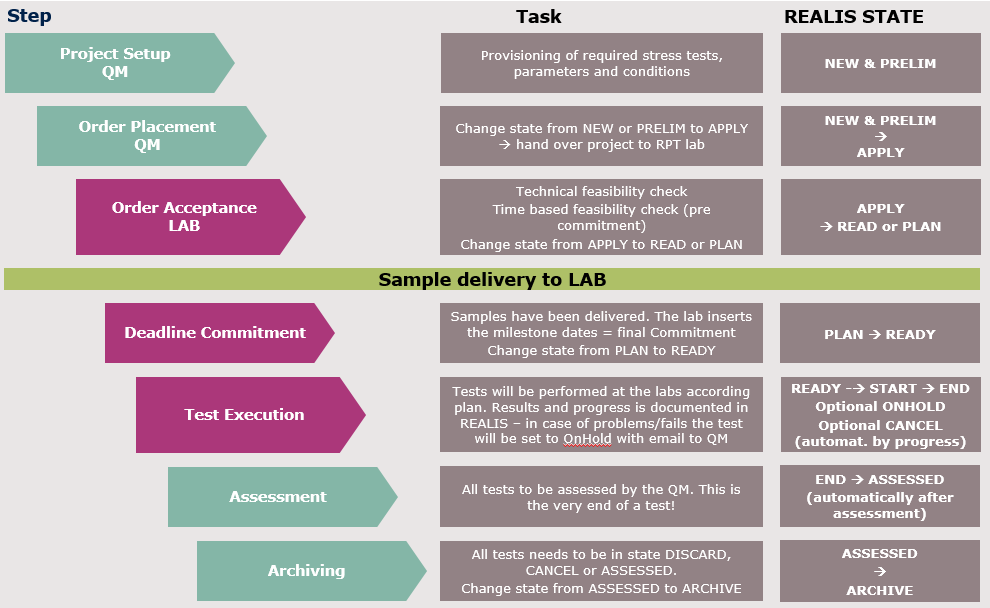
\includegraphics[width=1\textwidth]{bilder/realis-project-lifecycle.png}
    \caption{REALIS Project Lifecycle}
    \label{fig:realis-project-lifecycle}
\end{figure}

Anschließend wird ein Sample, also eine kleine Stückzahl des Produktes zum beauftragten \ac{RPT}-Labor geschickt. Dieses wird in der Fachsprache auch als Test-Los, oder zu Englisch: \textit{test lot}
bezeichnet. Die Stückzahl wird dabei in \ac{REALIS} dokumentiert. Die  Daten der Testoperation werden dann final festgelegt und der Test Status wird geändert.

Daraufhin erfolgt die planmäßige Durchführung der einzelnen Operation der Stresstests. Dabei werden der Fortschritt und die Ergebnisse von Mitarbeitern in \ac{REALIS} dokumentiert. Treten während der Stresstests Probleme oder Fehler auf, werden diese an den \ac{QM} weitergeleitet, der anschließend über das weitere Vorgehen entscheidet.

Nachdem alle Tests vollständig durchgeführt und dokumentiert worden sind, muss der \ac{QM} die Ergebnisse prüfen und bewerten. Zum Schluss werden die Tests dann archiviert, womit der Project-Lifecycle beendet ist.

\subsection{Architektur und Technologie}
Das ursprüngliche Frontend von REALIS war eine Windows-Desktop-Applikation, die sowohl vom \ac{RPT}-Labor-Mitarbeiter als auch vom \ac{QM} genutzt wurde. Im Zuge einer Modernisierung wird das System schrittweise zu einer Web-Applikation migriert. Gleichzeitig erfolgt eine Aufteilung in zwei separate Systeme, um die unterschiedlichen Aufgabenbereiche des RPT-Labors und des \acp{QM} klar voneinander abzugrenzen.

Abbildung \ref{fig:realis-komponentendiagramm} zeigt die aktuelle Systemarchitektur in Form eines Komponentendiagramms. Im Backend (grün dargestellt) kommuniziert der \texttt{REALIS-Business-Layer} über eine \texttt{DataAccess}-Schnittstelle direkt mit der zentralen \texttt{REALIS-Datenbank} basierend auf Oracle. Der Business-Layer stellt die Geschäftslogik bereit und wird über eine \texttt{REST-API} von den Frontends genutzt.

\begin{figure}[!h]
    \centering
    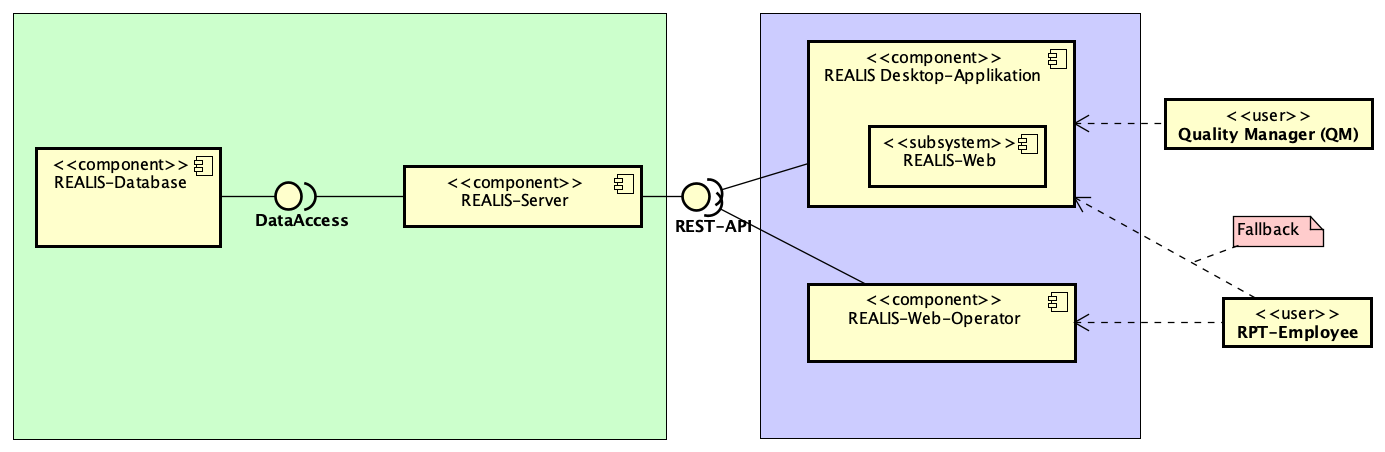
\includegraphics[width=1\textwidth]{bilder/REALIS-Komponentendiagramm.png}
    \caption{REALIS Komponentendiagramm}
    \label{fig:realis-komponentendiagramm}
\end{figure}

Das Frontend besteht aus zwei Hauptkomponenten (blau dargestellt):
\begin{enumerate}
    \item \textbf{REALIS-Desktop-Applikation:} \\
Die ursprüngliche Desktop-Anwendung, die sukzessive durch die Integration von neuen Web-Funktionalitäten modernisiert wird. Diese Web-Module, die mit Angular entwickelt werden, sind als Subsystem (\texttt{REALIS-Web}) innerhalb der Desktop-Applikation eingebettet. Dieses System steht sowohl dem \ac{QM} als auch dem \ac{RPT}-Labor-Mitarbeiter zur Verfügung. Langfristig wird der \ac{RPT}-Labor-Mitarbeiter jedoch keinen Zugriff mehr darauf haben.

\item \textbf{REALIS-Web-Operator-System:} \\
Eine eigenständige Web-Applikation, die speziell für die Anforderungen des \ac{RPT}-Labors entwickelt wird. Diese Anwendung befindet sich noch in der Entwicklung, wird jedoch bereits für einige Aufgaben eingesetzt. Für nicht implementierte Funktionen muss der \ac{RPT}-Mitarbeiter vorübergehend auf die alte Desktop-Applikation ausweichen. Zusätzlich ist geplant, das \texttt{REALIS-Web-Operator-System} als native iOS-App für mobile Apple-Geräte (z. B. iPads, iPhones) bereitzustellen. Die Verwendung von Angular ermöglicht dabei eine plattformübergreifende Entwicklung, die sowohl als Web-App als auch als native App funktioniert.
\end{enumerate}

Das Diagramm verdeutlicht die Trennung zwischen Backend und Frontend sowie die unterschiedlichen Nutzerrollen (\ac{QM} und \ac{RPT}-Labor-Mitarbeiter), die spezifische Zugriffsrechte auf die jeweiligen Systeme haben.


\subsection{Weitere Funktionen und Statistiken}
\ac{REALIS} bietet über das Anlegen von Zuverlässigkeitstests (Reliability-Tests) hinaus zusätzliche Funktionen, um Prozesse effizienter zu gestalten und Engpässe zu vermeiden. So ermöglicht das System beispielsweise die Planung individueller Laborkapazitäten, wodurch unnötige Investitionen vermieden werden können. Zudem erlaubt es die Referenzierung bereits durchgeführter Testergebnisse, um doppelte Tests zu vermeiden.

Nach Abschluss eines Tests können in \ac{REALIS} automatisch benötigte Ergebnisberichte generiert werden – sowohl für den Kunden als auch für das \ac{RPT}-Labor. Dies erleichtert die Dokumentation und erhöht die Effizienz im Testmanagement.

Seit 2001 wird \ac{REALIS} erfolgreich genutzt. Derzeit arbeiten etwa 4.300 aktive Nutzer mit dem System. Es wird in 101 \ac{RPT}-Laboren in 17 verschiedenen Ländern eingesetzt. Aktuell verwaltet \ac{REALIS} rund 270.000 Projekte, mit etwa 1,9 Millionen Stresstests.